\documentclass{article}
\usepackage{cmap}
\usepackage[utf8]{inputenc}
\usepackage[english,ukrainian]{babel}
\usepackage{graphicx}
\usepackage{geometry}
\usepackage{listings}
\usepackage{float}
\usepackage{amsmath}
\geometry{
	a4paper,
	left=20mm,
	right=20mm,
	top=15mm,
	bottom=15mm,
}
\lstset{
	language=c,
	tabsize=4,
	keepspaces,
	showstringspaces=false,
}
\graphicspath{ {./pictures} }
\setlength{\parindent}{4em}

\newcommand\subject{Програмування в Інтернет}
\newcommand\lecturer{асистент кафедри ПЗ \\ Степанов Д.С.}
\newcommand\teacher{доцент кафедри ПЗ \\ Грицай О.Д.}
\newcommand\mygroup{ПЗ-22}
\newcommand\lab{2}
\newcommand\theme{Форма як головний елемент динаміки та зворотнього зв’язку з сервером}
\newcommand\purpose{Оволодіти засобами керування формами, внесення інформації для сервера на
	динамічній web-сторінці, ознайомитись з функціями JavaScript та бібліотеки jQuery}

\begin{document}
\begin{normalsize}
\begin{titlepage}
	\thispagestyle{empty}
	\begin{center}
		\textbf{МІНІСТЕРСТВО ОСВІТИ І НАУКИ УКРАЇНИ\\
			НАЦІОНАЛЬНИЙ УНІВЕРСИТЕТ "ЛЬВІВСЬКА ПОЛІТЕХНІКА"}
	\end{center}
	\begin{flushright}
		\textbf{ІКНІ}\\
		Кафедра \textbf{ПЗ}
	\end{flushright}
	\vspace{200pt}
	\begin{center}
		\textbf{ЗВІТ}\\
		\vspace{10pt}
		до лабораторної роботи № \lab\\
		\textbf{на тему}: “\textit{\theme}”\\
		\textbf{з дисципліни}: “\subject”
	\end{center}
	\vspace{112pt}
	\begin{flushright}
		
		\textbf{Лектор}:\\
		\lecturer\\
		\vspace{28pt}
		\textbf{Виконав}:\\
		
		студент групи \mygroup\\
		Коваленко Д.М.\\
		\vspace{28pt}
		\textbf{Прийняв}:\\
		
		\teacher\\
		
		\vspace{28pt}
		«\rule{1cm}{0.15mm}» \rule{1.5cm}{0.15mm} 2023 р.\\
		$\sum$ = \rule{1cm}{0.15mm}……………\\
		
	\end{flushright}
	\vspace{\fill}
	\begin{center}
		\textbf{Львів — 2023}
	\end{center}
\end{titlepage}
	
\begin{description}
	\item[Тема.] \theme.
	\item[Мета.] \purpose.
\end{description}

\section*{Індивідуальне завдання}
Розробити web-сторінку згідно макета (wireframe)
https://cacoo.com/diagrams/ZvVhYS3UpG5PdbBy/EDE3A
Обираємо для розробки шаблон Students Add/Edit
Використовуємо Gitlab (https://gitlab.com)
Сторінка має містити:\\
- модальне вікно для внесення даних як на макеті з прихованим полем id\\
- для редагування даних використовується те саме вікно\\
- кнопки у модальному вікні та реакції на ці кнопки функціями JavaScript/jQuery.\\
- функція додавання/збереження має сформувати рядок даних, що буде передаватись\\
з даної форми на сервер.\\
- створити стандартний опис з будь яким кешуванням PWA

\section*{Теоретичні відомості}
Одним з інструментів підтримки динамічних сценаріїв при перегляді Web-сторінок у
межах комп’ютера користувача є мова програмування JavaScript – спрощений
варіант мови програмування Java. Нею запезпечується рух об’єктів на сторінці,
введення та виведення параметрів, зміна зображень вікон тощо. Програми модифікації,
створення гіпертекстових сторінок традиційно називають скриптами (scripts), які
інтерпретуються програмою перегляду. Спосіб базується на ідеології об’єктно-
орієнтованого програмування. Зупинимось на скриптах, написаних мовою JavaScript.

Усі операції в програмі на JavaScript описують дії над об’єктами – елементами
робочої області броузера та контейнерами мови HTML. Об’єкти мають властивості та
методи. Існують також інші функції, які дають змогу працювати зі стандартними
математичними функціями та керувати процесом виконання програми. JavaScript має
механізм опрацювання подій перегляду динамічних об’єктів та управління
багатовіконним інтерфейсом. Об’єкти JavaScript беруть свій початок від класу
Window.

Bootstrap – це фреймворк для розробки клієнтських застосувань (front end). Bootstrap
містить шаблони на базі HTML та CSS з текстом, формами, кнопками, таблицями,
навігацією, модулями, каруселями зображень та багато інших сучасних елементів веб
сторінок, а також вбудовані засоби JavaScript (плагіни). Bootstrap дозволяє створювати
адаптивні сторінки у телефонах, планшетах та ноутбуках.. Bootstrap 3 підтримує
реалізацію для мобільних телефонів. Bootstrap підтримується у сучасних браузерах
(Chrome, Firefox, Internet Explorer, Safari, Opera). Версія 4.0 містить препроцесор CSS
(SASS ) та підтримку flex-box.

\section*{Хід виконання}
\begin{lstlisting}
let students = []
let globalStudentId = 1;
let studentIdToDelete = 0;
let studentIdToEdit = 0;
// Checkboxes
const checkAll = document.getElementById("check-all");

checkAll.addEventListener("click", () => {
	const checkboxes = document.querySelectorAll(".check");
	checkboxes.forEach((checkbox) => {
		checkbox.checked = checkAll.checked;
	});
});



// Delete row of table && warning modal
const warningModal = document.getElementById("warning-modal-wrapper");
const warningCloseBtn = document.getElementById("warning-modal-close");
const warningCancelBtn = document.getElementById("warning-modal-cancel");

warningCloseBtn.addEventListener('click', () => {
	warningModal.style.display = "none";
});

warningCancelBtn.addEventListener('click', () => {
	warningModal.style.display = "none";
});

const warningDeleteBtn = document.getElementById("warning-modal-delete");
warningDeleteBtn.addEventListener("click", () => {
	const i = students.findIndex(s => s.id === studentIdToDelete);
	students.splice(i, 1);
	clearTable();
	drawTable();
	warningModal.style.display = "none";
	studentIdToDelete = 0;
})


// Add row to table && add modal
const addBtn = document.getElementById("add-row");
const addModal = document.getElementById("add-modal-wrapper");
const addModalCloseBtn = document.getElementById("add-modal-close");
const addModalOkBtn = document.getElementById("add-modal-create");
const addForm = document.getElementById("add-form");

addBtn.addEventListener("click", () => {
	const a = document.getElementById("add-form-title");
	const b = document.getElementById("add-modal-create");
	a.innerHTML = "Add Student";
	b.innerHTML = "Add";
	addModal.style.display = "block";
})

addModalCloseBtn.addEventListener('click', () => {
	addModal.style.display = "none";
	addForm.reset();
});

function validateStudent(student) {
	valid = true;
	
	const fieldGroup = document.getElementById("add-form-field-group");
	const fieldFirstName = document.getElementById("add-form-field-firstName");
	const fieldLastName = document.getElementById("add-form-field-lastName");
	const fieldGender = document.getElementById("add-form-field-gender");
	const fieldBirthday = document.getElementById("add-form-field-birthday");
	
	if (student.name.split(" ")[0] === "") {
		fieldFirstName.classList.add("invalid");
		valid = false;
	} else {
		fieldFirstName.classList.remove("invalid");
	}
	
	if (student.name.split(" ")[1] === "") {
		fieldLastName.classList.add("invalid");
		valid = false;
	} else {
		fieldLastName.classList.remove("invalid");
	}
	
	const birthday = new Date(student.birthday);
	if (isNaN(birthday.getTime()) || birthday > new Date()) {
		fieldBirthday.classList.add("invalid");
		valid = false;
	} else {
		fieldBirthday.classList.remove("invalid");
	}
	return valid;
}

function addStudent() {
	const fieldId = document.getElementById("add-form-field-id");
	const fieldGroup = document.getElementById("add-form-field-group");
	const fieldFirstName = document.getElementById("add-form-field-firstName");
	const fieldLastName = document.getElementById("add-form-field-lastName");
	const fieldGender = document.getElementById("add-form-field-gender");
	const fieldBirthday = document.getElementById("add-form-field-birthday");
	const id = globalStudentId++;
	fieldId.value = id;
	const name = fieldFirstName.value + " " + fieldLastName.value;
	const group = fieldGroup.options[fieldGroup.selectedIndex].textContent;
	const gender = fieldGender.options[fieldGender.selectedIndex].textContent;
	const birthday = fieldBirthday.value;
	
	const student = {
		"id": id,
		"group": group,
		"name": name,
		"gender": gender,
		"birthday": birthday,
		"status": 1,
	};
	
	if (!validateStudent(student)) {
		return;
	}
	
	addModal.style.display = "none";
	
	students.push(student);
	
	clearTable();
	drawTable();
	addForm.reset();
	console.log(JSON.stringify(student));
}

function editStudent(studentId) {
	const i = students.findIndex(s => s.id === studentIdToEdit);
	const fieldId = document.getElementById("add-form-field-id");
	const fieldGroup = document.getElementById("add-form-field-group");
	const fieldFirstName = document.getElementById("add-form-field-firstName");
	const fieldLastName = document.getElementById("add-form-field-lastName");
	const fieldGender = document.getElementById("add-form-field-gender");
	const fieldBirthday = document.getElementById("add-form-field-birthday");
	const id = fieldId.value;
	const name = fieldFirstName.value + " " + fieldLastName.value;
	const group = fieldGroup.options[fieldGroup.selectedIndex].textContent;
	const gender = fieldGender.options[fieldGender.selectedIndex].textContent;
	const birthday = fieldBirthday.value;
	
	const student = {
		"id": id,
		"group": group,
		"name": name,
		"gender": gender,
		"birthday": birthday,
		"status": 1,
	};
	
	if (!validateStudent(student)) {
		return;
	}
	
	addModal.style.display = "none";
	
	students[i] = student;
	
	clearTable();
	drawTable();
	addForm.reset();
	console.log(JSON.stringify(student));
	studentIdToEdit = 0;
}

window.onclick = function (event) {
	if (event.target === addModal) {
		addModal.style.display = "none";
	}
};

addModalOkBtn.addEventListener('click', () => {
	const e = document.getElementById("add-form-title");
	if (e.innerHTML === "Edit Student") {
		editStudent();
	} else {
		addStudent();
	}
});

// Profile && notification headers
const profileHeaderTrigger = document.getElementById("profile-header-trigger");
const profileHeader = document.getElementById("profile-header");
const notificationHeaderTrigger = document.getElementById("notification-header-trigger");
const notificationHeader = document.getElementById("notification-header");

profileHeaderTrigger.addEventListener('mouseover', function () {
	profileHeader.classList.add('active');
});

profileHeader.addEventListener('mouseleave', function () {
	profileHeader.classList.remove('active');
});

document.addEventListener('click', function (event) {
	if (!profileHeaderTrigger.contains(event.target) && !profileHeader.contains(event.target)) {
		profileHeader.classList.remove('active');
	}
});

notificationHeaderTrigger.addEventListener('mouseover', function () {
	notificationHeader.classList.add('active');
});

notificationHeader.addEventListener('mouseleave', function () {
	notificationHeader.classList.remove('active');
});

document.addEventListener('click', function (event) {
	if (!notificationHeaderTrigger.contains(event.target) && !notificationHeader.contains(event.target)) {
		notificationHeader.classList.remove('active');
	}
});

function drawTable() {
	const table = document.getElementById("table");
	students.forEach((student) => {
		const newRow = table.insertRow();
		newRow.id = student.id;
		const checkboxCell = newRow.insertCell();
		const checkbox = document.createElement("input");
		checkbox.type = "checkbox";
		checkbox.className = "check";
		checkboxCell.appendChild(checkbox);
		
		const groupCell = newRow.insertCell();
		groupCell.textContent = student.group;
		
		const nameCell = newRow.insertCell();
		nameCell.innerHTML = student.name;
		
		const genderCell = newRow.insertCell();
		genderCell.textContent = student.gender;
		
		const dobCell = newRow.insertCell();
		dobCell.innerHTML = student.birthday;
		
		const statusCell = newRow.insertCell();
		const statusDiv = document.createElement("div");
		statusDiv.className = "status-active";
		statusCell.appendChild(statusDiv);
		
		const actionCell = newRow.insertCell();
		const editButton = document.createElement("button");
		editButton.className = "edit-row btn fa fa-edit";
		editButton.onclick = function () {
			studentIdToEdit = student.id;
			const a = document.getElementById("add-form-title");
			const b = document.getElementById("add-modal-create");
			a.innerHTML = "Edit Student";
			b.innerHTML = "Edit";
			addModal.style.display = "block";
			
			const fieldId = document.getElementById("add-form-field-id");
			fieldId.value = student.id;
			const fieldGroup = document.getElementById("add-form-field-group");
			for (let i = 0; i < fieldGroup.options.length; i++) {
				if (fieldGroup.options[i].text === student.group) {
					fieldGroup.selectedIndex = i;
					break;
				}
			}
			const fieldFirstName = document.getElementById("add-form-field-firstName");
			fieldFirstName.value = student.name.split(" ")[0];
			const fieldLastName = document.getElementById("add-form-field-lastName");
			fieldLastName.value = student.name.split(" ")[1];
			const fieldGender = document.getElementById("add-form-field-gender");
			for (let i = 0; i < fieldGender.options.length; i++) {
				if (fieldGender.options[i].text === student.gender) {
					fieldGender.selectedIndex = i;
					break;
				}
			}
			const fieldBirthday = document.getElementById("add-form-field-birthday");
			fieldBirthday.value = student.birthday;
			const name = fieldFirstName.value + " " + fieldLastName.value;
			const group = fieldGroup.options[fieldGroup.selectedIndex].textContent;
			const gender = fieldGender.options[fieldGender.selectedIndex].textContent;
			const birthday = fieldBirthday.value;
		};
		actionCell.appendChild(editButton);
		
		const deleteButton = document.createElement("button");
		deleteButton.className = "delete-row btn fa fa-remove";
		deleteButton.onclick = function() {
			warningModal.style.display = "block";
			studentIdToDelete = student.id;
		};
		actionCell.appendChild(deleteButton);
	});
}

function clearTable() {
	const table = document.getElementById("table");
	let rowCount = table.rows.length;
	for (let i = rowCount - 1; i > 0; i--) {
		table.deleteRow(i);
	}
}

\end{lstlisting}

\section*{Результати}
\begin{figure}[H]
	\centering
	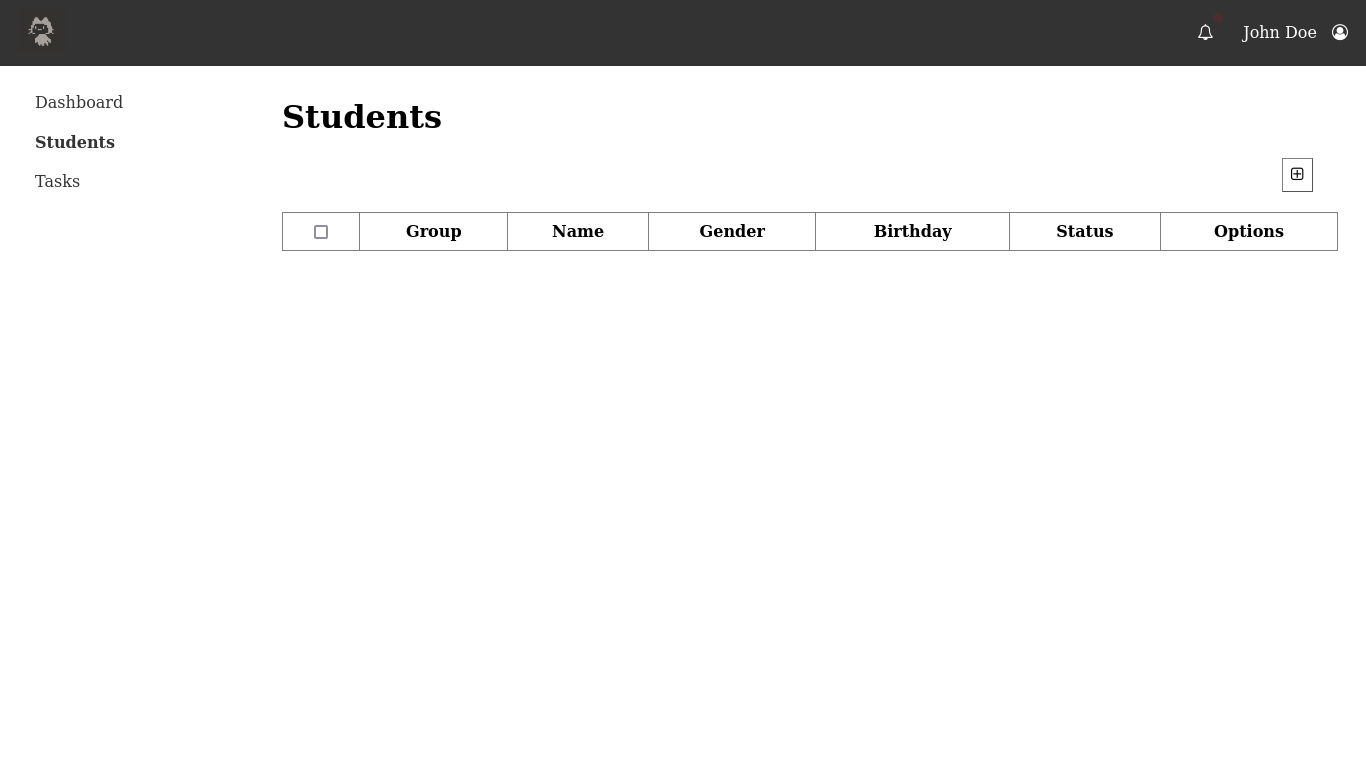
\includegraphics[scale=0.35]{1}
	\caption{Загальний вигляд сторінки}
\end{figure}

\begin{figure}[H]
	\centering
	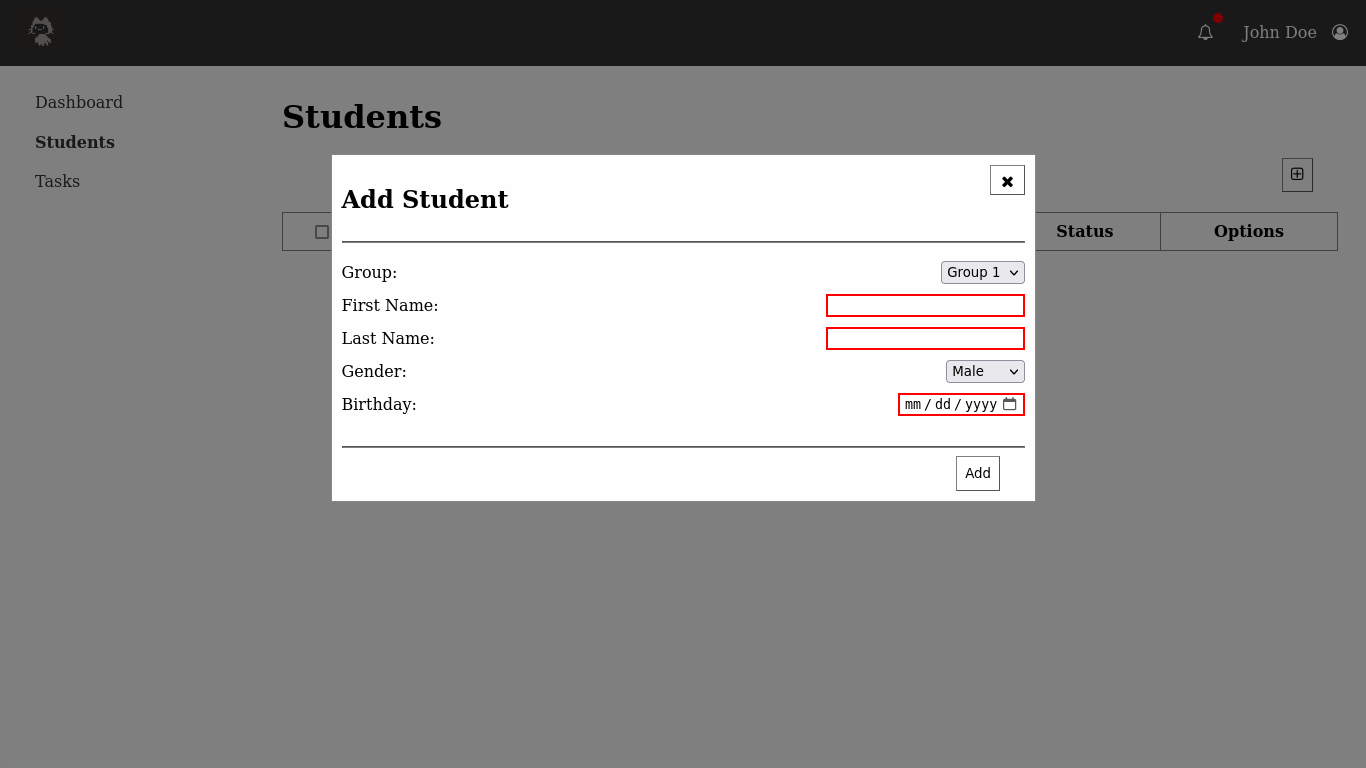
\includegraphics[scale=0.35]{3}
	\caption{Модальне вікно для додавання студента та його валідація}
\end{figure}

\begin{figure}[H]
	\centering
	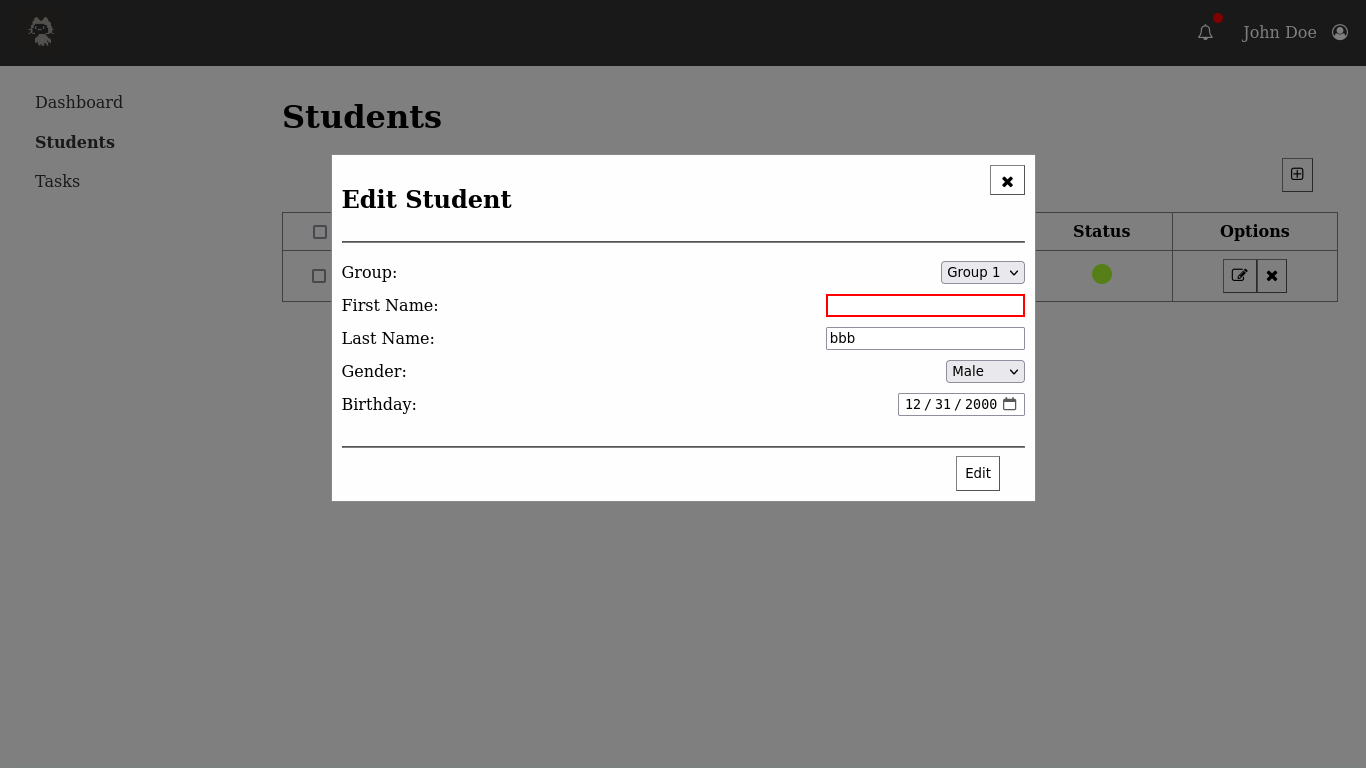
\includegraphics[scale=0.35]{6}
	\caption{Модальне вікно для видалення студента та його валідація}
\end{figure}

\begin{figure}[H]
	\centering
	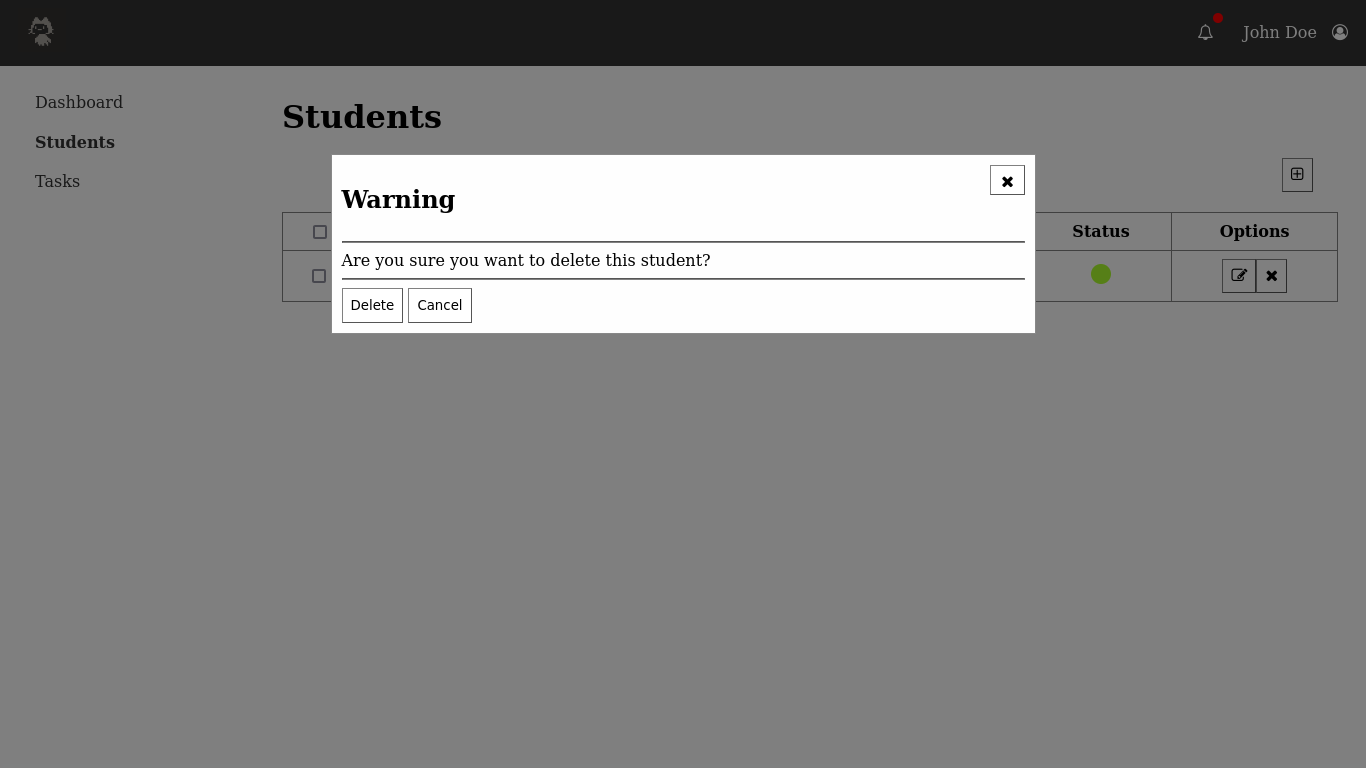
\includegraphics[scale=0.35]{7}
	\caption{Модальне вікно для видалення студента}
\end{figure}

\begin{figure}[H]
	\centering
	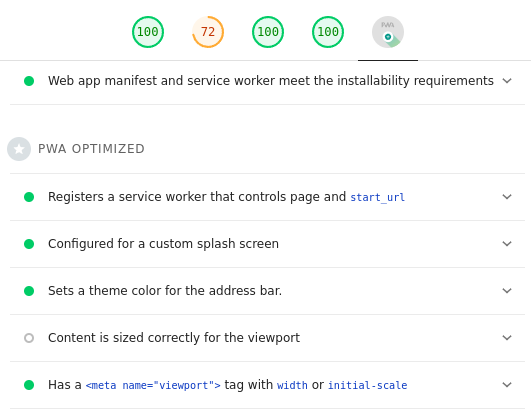
\includegraphics[scale=0.5]{10}
	\caption{Виконано PWA кешування}
\end{figure}

\section*{Висновки}
Під час виконання лабораторної роботи я оволодів засобами керування формами, внесення інформації для сервера на
динамічній web-сторінці, ознайомивя з функціями JavaScript та бібліотою jQuery.
	    
\end{normalsize}
\end{document}
